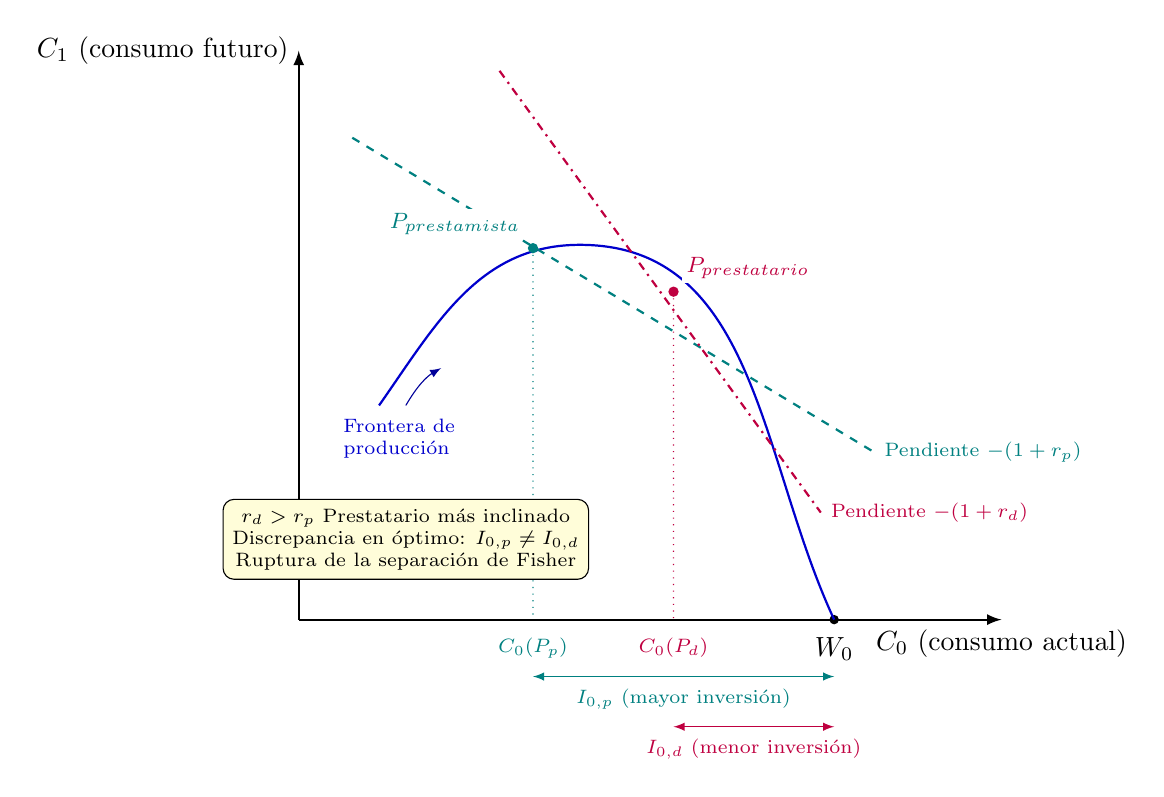
\begin{tikzpicture}[scale=0.85, >=latex]
  % Ejes
  \draw[->, thick] (0,0) -- (10.5,0) node[below] {$C_0$ (consumo actual)};
  \draw[->, thick] (0,0) -- (0,8.5) node[left] {$C_1$ (consumo futuro)};

  % Dotación inicial
  \coordinate (W) at (8,0);
  \fill (W) circle (2pt) node[below=3pt] {$W_0$};

  % Curva de producción real cóncava
  \draw[thick, blue!80!black] (8,0) to[out=115, in=0] (4.2,5.6) to[out=180, in=55] (1.2,3.2);
  \node[blue!80!black, font=\scriptsize, align=left] at (1.5, 2.7) {Frontera de\\producción};
  \draw[->, blue!60!black, shorten >=2pt] (1.6, 3.2) to[bend left=15] (2.2, 3.8);

  % Tangencia prestamista: r_prestamo (más baja -> recta más plana)
  \coordinate (Pp) at (3.5, 5.55);
  \draw[thick, teal, dashed] (0.8, 7.2) -- (8.6, 2.5) node[right, font=\scriptsize] {Pendiente $-(1+r_p)$};
  \fill[teal] (Pp) circle (2.2pt);
  \node[above left=3pt, font=\footnotesize, text=teal, fill=white, inner sep=1.5pt] at (3.5, 5.55) {$P_{\text{prestamista}}$};

  % Tangencia prestatario: r_endeudamiento (más alta -> recta más empinada)
  \coordinate (Pd) at (5.6, 4.9);
  \draw[thick, purple, dashdotted] (3.0, 8.2) -- (7.8, 1.6) node[right, font=\scriptsize] {Pendiente $-(1+r_d)$};
  \fill[purple] (Pd) circle (2.2pt);
  \node[above right=3pt, font=\footnotesize, text=purple, fill=white, inner sep=1.5pt] at (5.6, 4.9) {$P_{\text{prestatario}}$};

  % Proyecciones en eje C0
  \draw[dotted, teal] (Pp) -- (3.5,0) node[below=3pt, font=\scriptsize, text=teal] {$C_0(P_p)$};
  \draw[dotted, purple] (Pd) -- (5.6,0) node[below=3pt, font=\scriptsize, text=purple] {$C_0(P_d)$};

  % Cotas de inversión
  \draw[<->, teal] (3.5,-0.85) -- (8,-0.85) node[midway, below=1pt, font=\scriptsize] {$I_{0, p}$ (mayor inversión)};
  \draw[<->, purple] (5.6,-1.6) -- (8,-1.6) node[midway, below=1pt, font=\scriptsize] {$I_{0, d}$ (menor inversión)};

  % Nota explicativa en zona inferior izquierda bajo la curva (desplazada a x=1.6 para no tocar C0(Pp))
  \node[draw, rounded corners, fill=yellow!15, font=\scriptsize, align=center] at (1.6, 1.2) 
    {$r_d > r_p \implies$ Prestatario más inclinado\\
     Discrepancia en óptimo: $I_{0,p} \ne I_{0,d}$\\
     Ruptura de la separación de Fisher};
\end{tikzpicture}
